\documentclass[italian,a4paper]{article}
\usepackage[tight,nice]{units} %unità di misura
\usepackage{babel,amsmath,amssymb,amsthm,graphicx,url}
\usepackage[text={5.5in,9in},centering]{geometry}
\usepackage[utf8x]{inputenc}
\usepackage[T1]{fontenc}
\usepackage{ae,aecompl}
\usepackage{pstricks}
\usepackage[footnotesize,bf]{caption}
\usepackage{textcomp}
\usepackage{gensymb}
\frenchspacing
\pagestyle{plain}
%------------- eliminare prime e ultime linee isolate
\clubpenalty=9999%
\widowpenalty=9999
%--- definizione numerazioni
\renewcommand{\theequation}{\thesection.\arabic{equation}}
\renewcommand{\thefigure}{\arabic{figure}}
\renewcommand{\thetable}{\arabic{table}}
\addto\captionsitalian{\renewcommand{\figurename}{Grafico}}
%
%------------- ridefinizione simbolo per elenchi puntati: en dash
%\renewcommand{\labelitemi}{\textbf{--}}
\renewcommand{\labelenumi}{\textbf{\arabic{enumi}.}}
\setlength{\abovecaptionskip}{\baselineskip}   % 0.5cm as an example
\setlength{\floatsep}{2\baselineskip}
\setlength{\belowcaptionskip}{\baselineskip}   % 0.5cm as an example
%--------- comandi insiemi numeri complessi, naturali, reali e altre abbreviazioni
\renewcommand{\leq}{\leqslant}
%--------- porzione dedicata ai float in una pagina:
\renewcommand{\textfraction}{0.05}
\renewcommand{\topfraction}{0.95}
\renewcommand{\bottomfraction}{0.95}
\renewcommand{\floatpagefraction}{0.35}
\setcounter{totalnumber}{5}
%---------
%
%---------
\begin{document}
\title{Relazione di laboratorio: amplificatore}
\author{\normalsize Ilaria Brivio (582116)\\%
\normalsize \url{brivio.ilaria@tiscali.it}%
\and %
\normalsize Matteo Abis (584206)\\ %
\normalsize \url{webmaster@latinblog.org}
\and %
\normalsize Lorenzo Rossato (579393)\\ %
\normalsize \url{supergiovane05@hotmail.com}}
\date{\today}
\maketitle
%------------------
\noindent
Abbiamo costruito il circuito riportato in figura~\ref{fig:circuito}.
\begin{figure}[h]\caption{Rappresentazione schematica del circuito
    realizzato.}\label{fig:circuito}
    \centering
    \psset{unit=1in,cornersize=absolute,dimen=middle}%
\begin{pspicture}(-1.395,-0.9625)(0.383333,1.254722)%
% dpic version 16.Jan.09 for PSTricks 0.93a or later
\psset{linewidth=0.8pt}%
\psset{linewidth=0.8pt}%
\makeatletter\@ifundefined{MPSTPatchA}{\def\psbezier@ii{\addto@pscode{%
\ifshowpoints true \else false \fi\tx@OpenBezier%
\ifshowpoints\tx@BezierShowPoints\fi}\end@OpenObj}%
\global\def\MPSTPatchA{}}{}\makeatother%
\psset{arrowsize=1.1pt 4,arrowlength=1.64,arrowinset=0}%
\psline(0,0)(0,0.15)
(0,0.15)(-0.01107,0.15)
\psline(0,0.6)(0,0.45)
(0,0.45)(-0.01107,0.45)
\psline(-0.2,0.2)(-0.2,0.4)
\psline(-0.325,0.3)(-0.2,0.3)
\psline(0,0.15)(-0.2,0.24)
\psline[arrowsize=0.055556in 0,arrowlength=1.5,arrowinset=0]{<-}(-0.05,0.1725)(-0.15,0.2175)
\psline(0,0.45)(-0.2,0.36)
\psline(0,0.6)(0,0.775)
(0,0.775)(-0.041667,0.795833)
(-0.041667,0.795833)(0.041667,0.8375)
(0.041667,0.8375)(-0.041667,0.879167)
(-0.041667,0.879167)(0.041667,0.920833)
(0.041667,0.920833)(-0.041667,0.9625)
(-0.041667,0.9625)(0.041667,1.004167)
(0.041667,1.004167)(0,1.025)
(0,1.025)(0,1.2)
\uput{0.501875ex}[r](0.041667,0.9){\rlap{$ R_c$}}
\pscircle[fillstyle=solid,fillcolor=black](0,0.6){0.02}
\uput{0.501875ex}[r](0.02,0.6){\rlap{$ V_\text{out}$}}
\pscircle[fillstyle=solid,fillcolor=black](0,1.2){0.02}
\uput{0.501875ex}[u](0,1.22){$ +\unit[15]{V}$}
\psline(-0.325,0.3)(-0.775,0.3)
\psline(-0.775,0.3)(-0.775,0.6)
\psline(-0.775,0.6)(-0.775,0.775)
(-0.775,0.775)(-0.816667,0.795833)
(-0.816667,0.795833)(-0.733333,0.8375)
(-0.733333,0.8375)(-0.816667,0.879167)
(-0.816667,0.879167)(-0.733333,0.920833)
(-0.733333,0.920833)(-0.816667,0.9625)
(-0.816667,0.9625)(-0.733333,1.004167)
(-0.733333,1.004167)(-0.775,1.025)
(-0.775,1.025)(-0.775,1.2)
\uput{0.501875ex}[r](-0.733333,0.9){\rlap{$ R_1$}}
\pscircle[fillstyle=solid,fillcolor=black](-0.775,1.2){0.02}
\uput{0.501875ex}[u](-0.775,1.22){$ +\unit[15]{V}$}
\psline(-0.775,0.3)(-0.775,0)
\psline(-0.775,0)(-0.775,-0.325)
(-0.775,-0.325)(-0.733333,-0.345833)
(-0.733333,-0.345833)(-0.816667,-0.3875)
(-0.816667,-0.3875)(-0.733333,-0.429167)
(-0.733333,-0.429167)(-0.816667,-0.470833)
(-0.816667,-0.470833)(-0.733333,-0.5125)
(-0.733333,-0.5125)(-0.816667,-0.554167)
(-0.816667,-0.554167)(-0.775,-0.575)
(-0.775,-0.575)(-0.775,-0.9)
\uput{0.501875ex}[r](-0.733333,-0.45){\rlap{$ R_2$}}
\psline(-0.691667,-0.9)(-0.858333,-0.9)
\psline(-0.719444,-0.93125)(-0.830556,-0.93125)
\psline(-0.739286,-0.9625)(-0.810714,-0.9625)
\psline(-0.775,0.3)(-1.05,0.3)
\psline(-1.05,0.383333)(-1.05,0.216667)
\psline(-1.1,0.383333)(-1.1,0.216667)
\psline(-1.1,0.3)(-1.375,0.3)
\uput{0.501875ex}[u](-1.075,0.383333){$ C_1$}
\pscircle[fillstyle=solid,fillcolor=black](-1.375,0.3){0.02}
\uput{0.501875ex}[d](-1.375,0.28){$ V_\text{in}$}
\psline(0,0)(-0,-0.1)
(-0,-0.1)(0.041667,-0.120833)
(0.041667,-0.120833)(-0.041667,-0.1625)
(-0.041667,-0.1625)(0.041667,-0.204167)
(0.041667,-0.204167)(-0.041667,-0.245833)
(-0.041667,-0.245833)(0.041667,-0.2875)
(0.041667,-0.2875)(-0.041667,-0.329167)
(-0.041667,-0.329167)(0,-0.35)
(0,-0.35)(0,-0.45)
\uput{0.501875ex}[l](-0.125,-0.225){\llap{$ R_{e1}$}}
\psline(0,-0.45)(-0,-0.55)
(-0,-0.55)(0.041667,-0.570833)
(0.041667,-0.570833)(-0.041667,-0.6125)
(-0.041667,-0.6125)(0.041667,-0.654167)
(0.041667,-0.654167)(-0.041667,-0.695833)
(-0.041667,-0.695833)(0.041667,-0.7375)
(0.041667,-0.7375)(-0.041667,-0.779167)
(-0.041667,-0.779167)(0,-0.8)
(0,-0.8)(0,-0.9)
\uput{0.501875ex}[l](-0.125,-0.675){\llap{$ R_{e2}$}}
\psline(0.083333,-0.9)(-0.083333,-0.9)
\psline(0.055556,-0.93125)(-0.055556,-0.93125)
\psline(0.035714,-0.9625)(-0.035714,-0.9625)
\psline(0,-0.45)(0.3,-0.45)
\psline(0.3,-0.45)(0.3,-0.65)
\psline(0.216667,-0.65)(0.383333,-0.65)
\psline(0.216667,-0.7)(0.383333,-0.7)
\psline(0.3,-0.7)(0.3,-0.9)
\uput{0.501875ex}[ur](0.325,-0.675){\rlap{$ C_2$}}
\psline(0.383333,-0.9)(0.216667,-0.9)
\psline(0.355556,-0.93125)(0.244444,-0.93125)
\psline(0.335714,-0.9625)(0.264286,-0.9625)
\end{pspicture}%

\end{figure}
Si dovevano dimensionare le resistenze $R_1$, $R_2$, $R_{e1}$, $R_{e2}$,
$Rc$, $C_1$ e $C_2$
in modo che, in corrente continua, la corrente di collettore $I_c$ non
dipendesse da $\beta$ ed inoltre si avesse $\unit[15]{V}-V_{\text{out}} \sim V_{\text{out}}-
V_e = \unit[6]{V}$, mentre, in corrente alternata, si ottenesse un guadagno
$A={V_\text{out}}/{V_\text{in}}=-25$ e la frequenza di taglio inferiore fosse
$\unit[20]{kHz}$ (poniamo una frequenza di taglio per $C_2$ in modo tale che
fosse molto minore di quella definita da $C_1$).
Poniamo:
\begin{equation*}
     R_p= \dfrac{R_1 R_2}{R_1+R_2} \qquad R_e =R_{e1}+R_{e2}
\end{equation*}
Per $R_1$ e $R_2$ si deve avere
\begin{equation*}
    \begin{cases}
  R_p &\ll \beta R_e\\   
  \unit[50]{\ohm} &\ll R_p \ll \unit[500]{k\ohm} \\   
    \end{cases}
\end{equation*}
dove la seconda equazione è dettata dal fatto che altrimenti il segnale
varierebbe molto con l'amplificatore e quindi uscirebbe dalla zona
lineare.
per $R_{e1}$ e $R_{e2}$ si deve avere 
$I_c = \unit[2]{mA}$ e $\unit[15]{V}-V_{\text{out}} \sim
V_{\text{out}}- V_e = \unit[6]{V}$.
Infine, bisogna soddisfare le condizioni
\begin{align*}
  \frac{1}{2\pi R_p C_1} &= \unit[20]{kHz}\\  
 \frac{1}{2 \pi R_{e1} C_2} &\ll \unit[20]{kHz}\\
\end{align*}

Abbiamo dimensionato gli elementi del circuito nel modo seguente:
\begin{align*}
    R_1 &= \unit[15]{k\ohm}\\
    R_2 &= \unit[5.6]{k\ohm}\\
    R_c &= \unit[3.3]{k\ohm}\\
    R_{e1} &= \unit[120]{\ohm}\\
    R_{e2} &= \unit[1.5]{k\ohm}\\
    C_1 &= \unit[1.5]{nF}\\
    C_2 &= \unit[10]{\micro F}\\
\end{align*}
Con questi elementi ci aspettiamo infatti che la frequenza di taglio della
parte $R_{e1}C_2$ sia \unit[134]{Hz}, e quindi molto minore di
\unit[20]{kHz}.

Poi si ha $V_b = 15\cdot R_2/(R_1 +
R_2) = \unit[4.2]{V}$. Da ciò si ricava la corrente di emettitore, essendo $R_e =
\unit[1.62]{k\ohm}$, $I_e \sim I_c = (4.2-0.6)/1.62 = \unit[2.2]{mA}$.

Questi dati ci permettono di stimare infine il valor medio del potenziale $V_\text{out}
= 15 - 3.6\cdot R_c/R_e = \unit[7.7]{V}$. Questo valore è circa un V più
basso del necessario, per via delle dimensioni disponibili sulle
resistenze del partitore e di collettore. Per assicurarci dunque che il
transistor rimanga in zona lineare abbiamo leggermente aumentato la
tensione continua d'ingresso da \unit[15]{V} a \unit[15.7]{V}.

In tensione continua \unit[15.7]{V} abbiamo misurato la tensione di
collettore $V_c = \unit[8.64]{V}$, emettitore $V_e = \unit[3.60]{V}$ e base
$V_b = \unit[4.24]{V}$. Abbiamo trovato $\beta \sim 360$ nell'esperienza
precedente, e da questi valori si può ricavare l'impedenza
d'ingresso sulla parte variabile del segnale $h_{\text{ie}} = 0.025 / I_b =
0.025\beta R_c /(15.7-V_c) = \unit[4.2]{k\ohm}$ che è circa un decimo di
$\beta R_e$.

Il segnale d'ingresso $V_{\text{in}}$ è:
\begin{table}[h]
    \centering
    \begin{tabular}{rl}
        forma: & sinusoidale\\
        frequenza: & \unit[20]{kHz} $\sim$ \unit[3]{MHz}\\
        ampiezza pp: & \unit[200]{mV}\\
        valor medio: & \unit[0]{V}
    \end{tabular}
\end{table}\\
L'amplificazione attesa è in prima approssimazione $-R_c/(R_{e1}+R_{e2}) =
-27.5$. La misura effettuata (vedi grafico~\ref{fig:amplificazione}) risulta
$A = 22.1$, una stima teorica più accurata è:
\begin{equation*}
    A_t = -\dfrac{\beta R_c}{h_{\text{ie}} + (\beta +1)R_e} = 25.1
\end{equation*}
Abbiamo calcolato la frequenza di taglio inferiore attesa secondo le
dimensioni del condensatore $C_1$ e del parallelo di $R_1$ e $R_2$. Tale
frequenza di taglio risulta $f_{0,\text{inf}} = \unit[24.1]{kHz}$. La
frequenza di taglio superiore (l'amplificazione misurata a metà banda è
22.1, vedi grafico~\ref{fig:amplificazione}) invece dovrebbe essere $f_{0,\text{sup}} =
155/22.1 = \unit[7.0]{MHz}$. Abbiamo dunque registrato l'ampiezza dei
segnali in ingresso e in uscita a metà banda, ovvero intorno a
\unit[500]{kHz}, e poi vicino alle frequenze di taglio. I dati sono
riportati nella tabella~\ref{tab:amplificazione} e nel
grafico~\ref{fig:amplificazione}.
\begin{table}[h] \caption{Misure dell'amplificazione del segnale, a varie frequenze. La tolleranza sull'amplificazione è il 6\% del valore. Sono riportate le dimensioni della scala sull'oscilloscopio.}
    \label{tab:amplificazione}
    \centering
    \begin{tabular}{*3c r@{ $\pm$ }l}
    freq. (\unit[]{kHz}) &  $V_\text{in}$ (\unit[50]{mV}) & $ V_\text{out}$
    (\unit[500]{mV}) & \multicolumn{2}{c}{ampl.}\\
21.73  &  212   &  2.96  & 14.0 & 0.8\\
23.64   &  212  &  3.08  & 14.5 & 0.9\\
25.36   &  212  &  3.24  & 15.3 & 0.9\\
26.71   &  212  &  3.28  & 15.2 & 0.9\\
27.38   &  214  &  3.36  & 15.7 & 0.9\\
28.81   &  210  &  3.36  & 16.0 & 1.0\\
26.23   &  212  &  3.22  & 15.2 & 0.9\\
27.56   &  208  &  3.28  & 15.8 & 0.9\\
24.57   &  210  &  3.10  & 14.8 & 0.9\\
23.55   &  210  &  3.06  & 14.6 & 0.9\\
495.2  &  204  &  4.56  & 22.4 & 1.3\\
399.9  &  206  &  4.56  & 21.9 & 1.3\\
608.8  &  204  &  4.52  & 22.2 & 1.3\\
548.6  &  206  &  4.48  & 21.7 & 1.3\\
336.4  &  206  &  4.60  & 22.3 & 1.3\\
2416    &  196  &  3.36  & 17.1 & 1.0\\
2652   &  198  &  3.28  & 16.6 & 1.0\\
2753   &  200  &  3.20  & 16.4 & 1.0\\
2878   &  198  &  3.12  & 15.8 & 0.9\\
3060   &  196  &  3.02  & 15.4 & 0.9\\
3192   &  196  &  2.96  & 15.1 & 0.9\\
2944   &  196  &  3.08  & 15.7 & 0.9\\
2857   &  198  &  3.14  & 15.9 & 1.0\\
2886   &  198  &  3.16  & 16.0 & 1.0\\
2739   &  196  &  3.18  & 16.2 & 1.0\\
\end{tabular}
\end{table}\\
\begin{figure}[h]\caption{Grafico dell'amplificazione in funzione della
    frequenza, in scala logaritmica. Le barre di errore rappresentano la
    tolleranza del 6\%, le righe tratteggiate l'amplificazione a metà
    banda (in alto) e l'amplificazione di taglio.}
        \centering                                     
        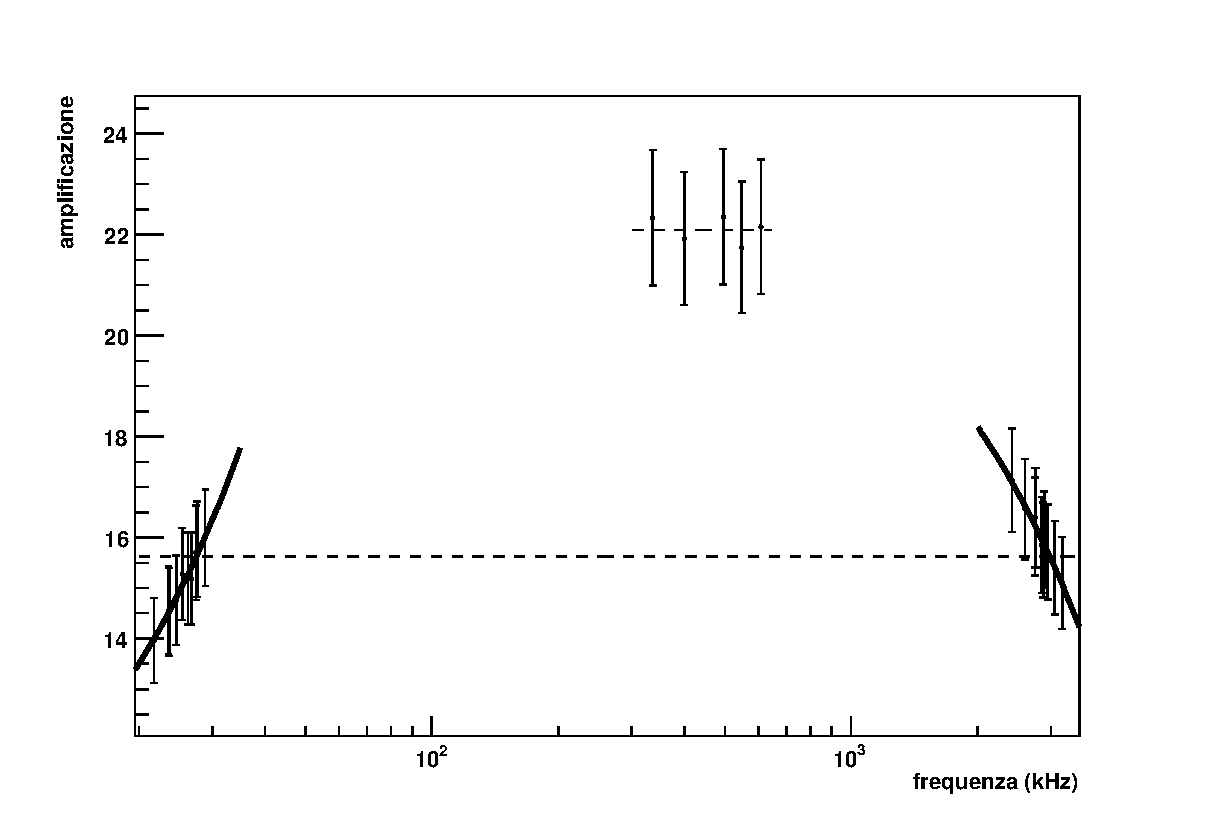
\includegraphics[width=\textwidth]{amplificazione.eps}
    \label{fig:amplificazione}
\end{figure}\\
Per trovare l'amplificazione abbiamo fatto la media dei valori registrati a
metà banda (retta tratteggiata più in alto nel grafico) e abbiamo ottenuto
dalle cinque misure
$A = 22.1 \pm 0.6$, con $\Delta A = 6\%A / \sqrt{5}$, perch\'e per ottenere
la tolleranza sulla media abbiamo diviso per la radice del numero delle
misure. La tolleranza
associata alla singola misura è del 6\% perch\'e le scale
sull'oscilloscopio sono diverse (vedi tabella) e quindi le tolleranze
del 3\% si
sommano linearmente. Abbiamo poi cercato
valori delle frequenze che realizzassero un'amplificazione di circa
$22.1/\sqrt{2} = 15.6$. Dai fit pesati delle misure intorno a tali frequenze
(vedi grafico~\ref{fig:amplificazione}) abbiamo trovato:
\begin{align*}
    f_{t,\text{inf}} &= \unit[27 \pm 3]{kHz}\\
    f_{t,\text{sup}} &= \unit[3.0 \pm 0.5]{MHz}\\
\end{align*}
Le tolleranze sono associate con un metodo grafico. La retta interpolante è
stata traslata verso l'alto e verso il basso di una quantità corrispondente
alla tolleranza sulle singole misure, ovvero il 6\% di 15.6 (ampiezza di
taglio). Metà della differenza tra le frequenze relative alle due
traslazioni è la tolleranza qui riportata.
Si nota che la frequenza di taglio inferiore è compatibile con il valore
atteso, mentre la frequenza di taglio superiore è molto lontana da
\unit[7]{MHz}. Ciò è dovuto al fatto che le misure sono state effettuate
con la sonda, che inserisce quindi in parallelo con l'impedenza di
uscita dell'amplificatore $Z_{\text{out}} \simeq R_c =
\unit[3.3]{k\ohm}$ una capacità di
circa $\unit[12]{pF}$. Tale circuito RC ha una frequenza di taglio di
$\unit[4]{MHz}$, ed è questa che determina il risultato delle misure. 
\subsection*{Emitter follower}
Connettere un emitter follower all'uscita del circuito precedente,
polarizzandolo con una corrente di circa \unit[10]{mA}. Verificare con
una misura che la frequenza di taglio inferiore rimane invariata.
Rimisurare la frequenza di taglio superiore e giustificare il fatto che
risulta maggiore di quella precedentemente misurata.

\begin{figure}[h]\caption{Rappresentazione schematica del circuito
    realizzato con l'emitter follower.}\label{fig:circuitoemitter}
    \centering
    \psset{unit=1in,cornersize=absolute,dimen=middle}%
\begin{pspicture}(-1.395,-0.9625)(1.084722,1.254722)%
% dpic version 16.Jan.09 for PSTricks 0.93a or later
\psset{linewidth=0.8pt}%
\psset{linewidth=0.8pt}%
\makeatletter\@ifundefined{MPSTPatchA}{\def\psbezier@ii{\addto@pscode{%
\ifshowpoints true \else false \fi\tx@OpenBezier%
\ifshowpoints\tx@BezierShowPoints\fi}\end@OpenObj}%
\global\def\MPSTPatchA{}}{}\makeatother%
\psset{arrowsize=1.1pt 4,arrowlength=1.64,arrowinset=0}%
\psline(0,0)(0,0.15)
(0,0.15)(-0.01107,0.15)
\psline(0,0.6)(0,0.45)
(0,0.45)(-0.01107,0.45)
\psline(-0.2,0.2)(-0.2,0.4)
\psline(-0.325,0.3)(-0.2,0.3)
\psline(0,0.15)(-0.2,0.24)
\psline[arrowsize=0.055556in 0,arrowlength=1.5,arrowinset=0]{<-}(-0.05,0.1725)(-0.15,0.2175)
\psline(0,0.45)(-0.2,0.36)
\psline(0,0.6)(0,0.775)
(0,0.775)(-0.041667,0.795833)
(-0.041667,0.795833)(0.041667,0.8375)
(0.041667,0.8375)(-0.041667,0.879167)
(-0.041667,0.879167)(0.041667,0.920833)
(0.041667,0.920833)(-0.041667,0.9625)
(-0.041667,0.9625)(0.041667,1.004167)
(0.041667,1.004167)(0,1.025)
(0,1.025)(0,1.2)
\uput{0.501875ex}[r](0.041667,0.9){\rlap{$ R_c$}}
\pscircle[fillstyle=solid,fillcolor=black](0,1.2){0.02}
\uput{0.501875ex}[u](0,1.22){$ V_{cc}$}
\psline(-0.325,0.3)(-0.775,0.3)
\psline(-0.775,0.3)(-0.775,0.6)
\psline(-0.775,0.6)(-0.775,0.775)
(-0.775,0.775)(-0.816667,0.795833)
(-0.816667,0.795833)(-0.733333,0.8375)
(-0.733333,0.8375)(-0.816667,0.879167)
(-0.816667,0.879167)(-0.733333,0.920833)
(-0.733333,0.920833)(-0.816667,0.9625)
(-0.816667,0.9625)(-0.733333,1.004167)
(-0.733333,1.004167)(-0.775,1.025)
(-0.775,1.025)(-0.775,1.2)
\uput{0.501875ex}[r](-0.733333,0.9){\rlap{$ R_1$}}
\pscircle[fillstyle=solid,fillcolor=black](-0.775,1.2){0.02}
\uput{0.501875ex}[u](-0.775,1.22){$ V_{cc}$}
\psline(-0.775,0.3)(-0.775,0)
\psline(-0.775,0)(-0.775,-0.325)
(-0.775,-0.325)(-0.733333,-0.345833)
(-0.733333,-0.345833)(-0.816667,-0.3875)
(-0.816667,-0.3875)(-0.733333,-0.429167)
(-0.733333,-0.429167)(-0.816667,-0.470833)
(-0.816667,-0.470833)(-0.733333,-0.5125)
(-0.733333,-0.5125)(-0.816667,-0.554167)
(-0.816667,-0.554167)(-0.775,-0.575)
(-0.775,-0.575)(-0.775,-0.9)
\uput{0.501875ex}[r](-0.733333,-0.45){\rlap{$ R_2$}}
\psline(-0.691667,-0.9)(-0.858333,-0.9)
\psline(-0.719444,-0.93125)(-0.830556,-0.93125)
\psline(-0.739286,-0.9625)(-0.810714,-0.9625)
\psline(-0.775,0.3)(-1.05,0.3)
\psline(-1.05,0.383333)(-1.05,0.216667)
\psline(-1.1,0.383333)(-1.1,0.216667)
\psline(-1.1,0.3)(-1.375,0.3)
\uput{0.501875ex}[u](-1.075,0.383333){$ C_1$}
\pscircle[fillstyle=solid,fillcolor=black](-1.375,0.3){0.02}
\uput{0.501875ex}[d](-1.375,0.28){$ V_\text{in}$}
\psline(0,0)(-0,-0.1)
(-0,-0.1)(0.041667,-0.120833)
(0.041667,-0.120833)(-0.041667,-0.1625)
(-0.041667,-0.1625)(0.041667,-0.204167)
(0.041667,-0.204167)(-0.041667,-0.245833)
(-0.041667,-0.245833)(0.041667,-0.2875)
(0.041667,-0.2875)(-0.041667,-0.329167)
(-0.041667,-0.329167)(0,-0.35)
(0,-0.35)(0,-0.45)
\uput{0.501875ex}[l](-0.125,-0.225){\llap{$ R_{e1}$}}
\psline(0,-0.45)(-0,-0.55)
(-0,-0.55)(0.041667,-0.570833)
(0.041667,-0.570833)(-0.041667,-0.6125)
(-0.041667,-0.6125)(0.041667,-0.654167)
(0.041667,-0.654167)(-0.041667,-0.695833)
(-0.041667,-0.695833)(0.041667,-0.7375)
(0.041667,-0.7375)(-0.041667,-0.779167)
(-0.041667,-0.779167)(0,-0.8)
(0,-0.8)(0,-0.9)
\uput{0.501875ex}[l](-0.125,-0.675){\llap{$ R_{e2}$}}
\psline(0.083333,-0.9)(-0.083333,-0.9)
\psline(0.055556,-0.93125)(-0.055556,-0.93125)
\psline(0.035714,-0.9625)(-0.035714,-0.9625)
\psline(0,-0.45)(0.3,-0.45)
\psline(0.3,-0.45)(0.3,-0.65)
\psline(0.216667,-0.65)(0.383333,-0.65)
\psline(0.216667,-0.7)(0.383333,-0.7)
\psline(0.3,-0.7)(0.3,-0.9)
\uput{0.501875ex}[ur](0.325,-0.675){\rlap{$ C_2$}}
\psline(0.383333,-0.9)(0.216667,-0.9)
\psline(0.355556,-0.93125)(0.244444,-0.93125)
\psline(0.335714,-0.9625)(0.264286,-0.9625)
\psline(0,0.6)(0.6,0.6)
\psline(0.925,0.35)(0.925,0.45)
(0.925,0.45)(0.91393,0.45)
\psline(0.925,0.85)(0.925,0.75)
(0.925,0.75)(0.91393,0.75)
\psline(0.725,0.5)(0.725,0.7)
\psline(0.6,0.6)(0.725,0.6)
\psline(0.925,0.45)(0.725,0.54)
\psline[arrowsize=0.055556in 0,arrowlength=1.5,arrowinset=0]{<-}(0.875,0.4725)(0.775,0.5175)
\psline(0.925,0.75)(0.725,0.66)
\pscircle[fillstyle=solid,fillcolor=black](0.925,0.35){0.02}
\uput{0.501875ex}[r](0.945,0.35){\rlap{$ V_{\text{out}}$}}
\psline(0.925,0.35)(0.925,0.175)
(0.925,0.175)(0.966667,0.154167)
(0.966667,0.154167)(0.883333,0.1125)
(0.883333,0.1125)(0.966667,0.070833)
(0.966667,0.070833)(0.883333,0.029167)
(0.883333,0.029167)(0.966667,-0.0125)
(0.966667,-0.0125)(0.883333,-0.054167)
(0.883333,-0.054167)(0.925,-0.075)
(0.925,-0.075)(0.925,-0.25)
\uput{0.501875ex}[r](1.05,0.05){\rlap{$ R_{e3}$}}
\psline(1.008333,-0.25)(0.841667,-0.25)
\psline(0.980556,-0.28125)(0.869444,-0.28125)
\psline(0.960714,-0.3125)(0.889286,-0.3125)
\psline(0.925,0.85)(0.925,1.15)
\pscircle[fillstyle=solid,fillcolor=black](0.925,1.15){0.02}
\uput{0.501875ex}[u](0.925,1.17){$ V_{cc}$}
\end{pspicture}%

\end{figure}

Per ottenere il valore di corrente richiesta abbiamo inserito una
resistenza $R_{e3} = \unit[800]{\ohm}$ essendo dalle misure in corrente
continua eseguite nella parte precedente $V_c = \unit[8.64]{V}$, quindi
 abbiamo $V_{\text{out}} = V_c - \unit[0.6]{V} = \unit[8]{V} =
 \unit[10]{mA}\cdot \unit[0.8]{k\ohm}$.

 Abbiamo misurato l'amplificazione vicino alla frequenza di taglio inferiore
 precedentemente ricavata:
 \begin{table}[h]
     \centering
 \begin{tabular}{*4c}                                   
     freq. & $V_\text{in}$ & $V_\text{out}$ & ampl. \\
     \unit[27.61]{kHz} & \unit[186]{mV} & \unit[2.88]{V} & 15.5 $\pm$ 0.9 \\
 \end{tabular}
 \end{table}\\
 questa misura conferma che la frequenza di taglio inferiore è rimasta
 invariata, nella tolleranza delle misure.
 Al contrario, la frequenza di taglio superiore risulta:
 \begin{equation*}
     f_t = \unit[4.6 \pm 0.6]{MHz}
 \end{equation*}
\begin{figure}[h]\caption{Grafico dell'amplificazione in funzione della
    frequenza, vicino alla frequenza di taglio superiore, con l'emitter
    follower. Le barre di errore rappresentano la
    tolleranza del 6\%, la riga tratteggiata l'amplificazione di taglio.}
        \centering                                     
        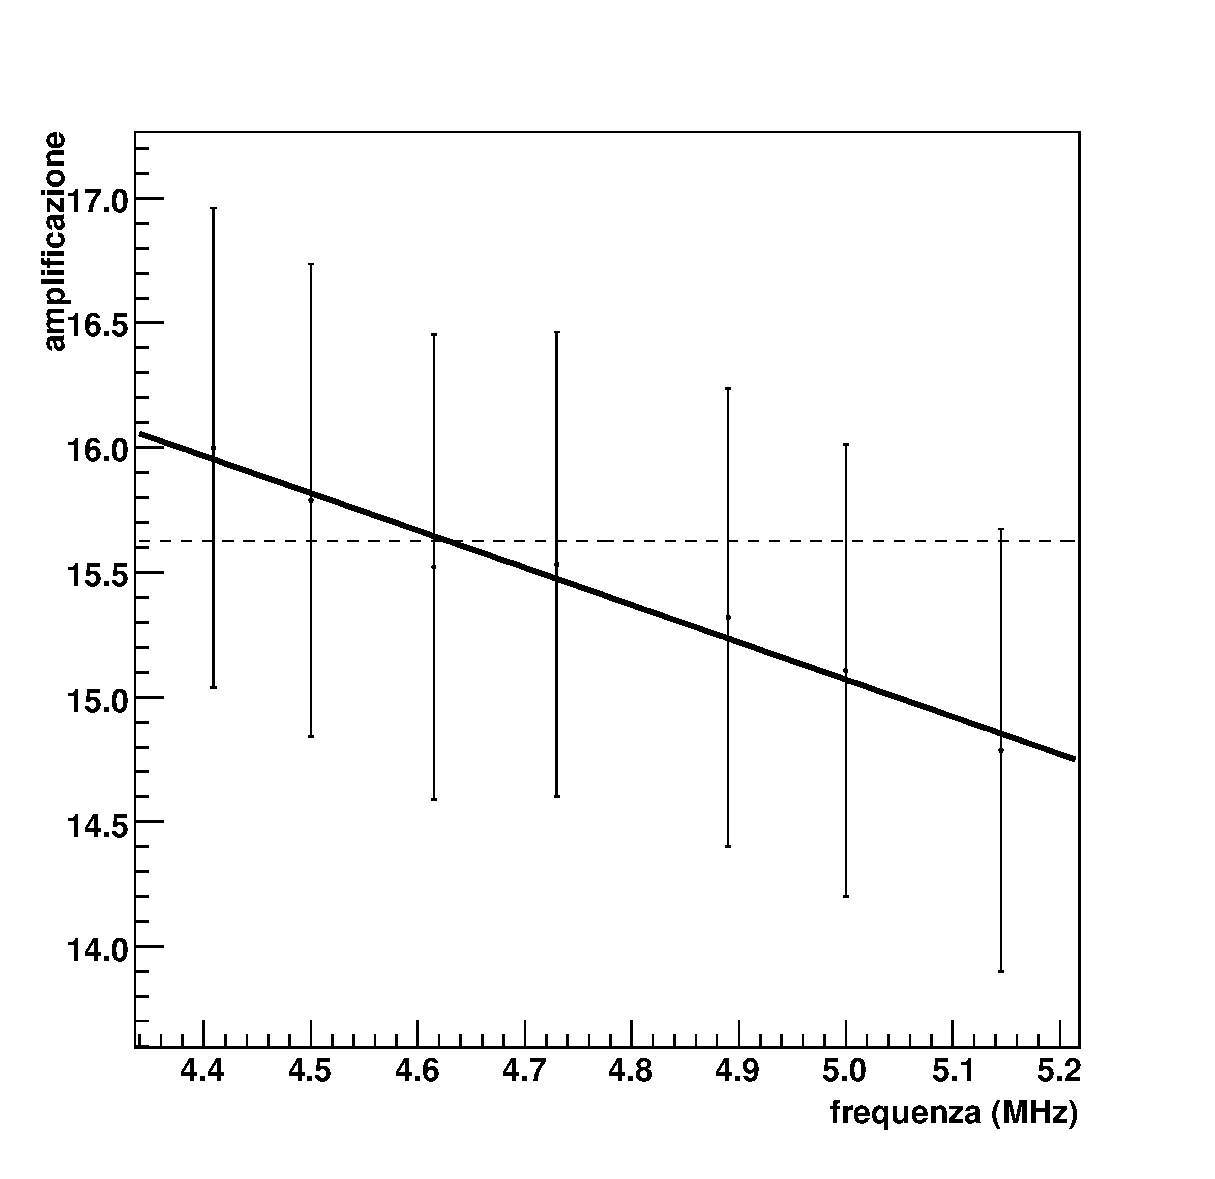
\includegraphics[width=0.7\textwidth]{emitter.eps}
    \label{fig:emitter}
\end{figure}\\
 Infatti l'impedenza di uscita dell'emitter follower è circa
 l'impedenza di uscita dell'amplificatore ridotta di un fattore $\beta$. La
 frequenza di taglio del circuito equivalente che comprende anche la sonda è
 dunque moltiplicata dello stesso fattore $\beta$, e risulta molto lontana
 dal valore atteso della frequenza di taglio superiore dell'amplificatore. 

 Si nota dunque che la nuova determinazione della frequenza di taglio è
 più vicina al valore atteso, anche se rimane una differenza non
 giustificabile con le sole tolleranze sulle misure.
\end{document}
